\documentclass[12pt]{article}
\usepackage{wrapfig}
\usepackage{graphicx}
\usepackage{epsfig}
\usepackage{url}
\usepackage{listings}
\usepackage{color}
\usepackage[left=2cm,top=1.5cm,right=2.5cm,bottom=1cm]{geometry}
\setlength{\parskip}{5mm plus5mm minus2mm}
\setlength{\parindent}{0mm}

\begin{document}

\title{Machine learning optimal parameters for a channel breakout system for trading
commodities}
\author{Martin Neal\\
  Becky Engley}
\date{\today}
\maketitle

\section{Introduction}

The commodities market is an exchange where raw materials and agricultural
products are traded. Commodities are usually traded via futures contracts. A
farmer can sell a futures contract on his crop, months or even years in advance
of the harvest, guaranteeing the price he will recieve at harvest time. A
grocery chain can buy the contract, with the confidence that the price will not
go up when the farmer delivers. Futures contracts protect farmers and buyers
from unexpected price changes.

Investors can also buy and sell the futures contracts, attempting to capitalize
on increases and decreases in price. If an investor expects an increase in the
value of a commodity, he will buy a contract while the price is low, and then
sell his contract at a later time, when the price is higher. In addition to
buying before selling, it is also possible to sell a contract before buying it
back, which an investor may do if he expects a commoditiy's value to decrease.
Buying before selling is referred to as \emph{trading long}; selling before
buying is known as \emph{trading short}.

It is often difficult for investors to determine when to buy and when to sell.
For example, it is impossible to recognize a minimum in price, until after the
price has increased above the minimum. Investors are left guessing as to
whether the price will continue to increase, or immediately begin decreasing
again. Guessing often proves to be unprofitable.

Momsen describes an automated trading system that attempts to predict trends in
commodity prices, providing the investor with a guide to buying and selling.
Momsen defines a pair of channel lines above and below the commodity's price.
The lines are defined using the price history. When the commodity's value
undergoes a change in trend, it crosses one of the channel lines, alerting the
investor to the change. At this point, the investor can decide to buy or
sell, appropriately.

Momsen's channel breakout system relies on a set of six parameters to define
the channel lines and date ranges between which an investor may buy and sell.
This paper aims to data mine commodity market prices, in order to learn better
parameters for Momsen's system. We use two machine learning algorithms to
search the parameter space; simulated annealing, and a genetic algorithm.

\vspace{-15pt}

\section{Related Work}

\vspace{-5pt}

Momsen's book, Superstar Seasonals, describes his channel breakout system as a
model for predicting uptrends and downtrends.  According to his system, a
commodity may be traded between a range of dates specified by the static
parameters $entry\_window\_open$ and $entry\_window\_close$.  A trade must be
completed no later than the $exit\_trade$ date, a third parameter of the
system.

Momsen defines an upper channel line and a lower channel line.  The upper
channel line is determined by the maximum high value over the previous m days.
The lower channel line is determined by the minimum low value over the previous
n days.  Here, m and n are also parameters of the system and are different for
each commodity.  If trading long, the upper channel line is the entry line, and
m is referred to as the $entry\_threshold$. The lower channel line is the
trail-stop line, and n is referred to as the $trail\_stop\_threshold$.  If
trading short, the channel lines are reversed.

The sixth and final system parameter, the $stop\_loss\_threshold$, serves as a
safety net to prevent large losses.  When trading short, the stop-loss is
defined by the maximum high value over the previous q days.  When trading long,
the stop-loss is defined by the minimum low value over the previous q days.  The
trail-stop line protects profits, while the stop-loss line minimizes losses.

According to the system, if the current value of the commodity crosses the entry
line, it indicates the beginning of a new trend, and the trade is begun.  When
the current value of the commodity crosses the trail-stop line, the trade is
completed.  More often than not, the cross of a channel line incorrectly
predicts the beginning of a new trend.  In these cases, small losses are incurred.
However, when the system correctly predicts a long trend, the profits generated
far outweigh small losses.

Over the past thirty years, Momsen has traded this system, with outstanding
results.  We extend his work by machine learning optimal values for the six
trading parameters.

\section{Methods}

Local search algorithms are used to maximize an objective function. Our
objective function is our algorithm for the channel breakout system, which
takes the six trading parameters as input, and returns the profit
earned. Optimal parameters maximize the profit earned as a result of trading the
system. We first discuss the algorithm for our objective function. Then, we
present the search algorithms that we use to explore the parameter space.

\subsection{Trading the System}

The channel breakout system processes financial market data for an individual
commodity, over a single contract year.  We describe our algorithm for the
channel breakout system below, along with our data set.

\vspace{25pt}
\subsubsection{Data Set}

We have financial market data for fourteen commodities over a period of thirty
years.  Because the learning system is evaluated per contract year, each year
comprises a single data point.  We have approximately thirty data points for
each commodity.  The commodities include live cattle, pork bellies, corn,
wheat, lean hogs, crude oil, unleaded gasoline, heating oil, and orange juice.
Some commodities are traded during multiple seasons.  The data includes open,
high, low, and closing values for each commodity for every trading day.

The data set is partitioned into two sets. For each commodity, we reserve one
third of the data points for testing; the remaining two thirds are used to train
the system. We use the earlier years of data for training, and the more recent
years for testing. We do not reserve any data for validation, as we do not need
to validate our predetermined model.

\subsubsection{The Channel Breakout System}

The algorithm for the channel breakout system takes in the six trading
parameters, and returns the total profit earned. Our $TradeSystem()$ function
is our objective function, the return value of which we are trying to maximize.
It is used as the $value()$ function for the Simulated Annealing algorithm, and
the $fitness()$ function for the Genetic algorithm, both defined in a later
section.
\vspace{25pt}

\setlength{\parindent}{5mm}
\indent TradeSystem(entry\_window\_open, entry\_window\_close, exit\_date,\\
\indent \indent \indent \indent \indent entry\_threshold, trail\_stop\_threshold, stop\_loss\_threshold)\\\\
\indent \indent compute entry, trail\_stop and stop\_loss channels, using thresholds\\\\
\indent \indent while(entry\_window\_open $<$ current\_date $<$ entry\_window\_close OR in\_trade)\\
\indent \indent \indent if(not in\_trade)\\
\indent \indent \indent \indent if(entry\_channel is crossed)\\
\indent \indent \indent \indent \indent in\_trade $\leftarrow$ TRUE\\
\indent \indent \indent \indent \indent entry\_price $\leftarrow$ current\_price\\
\indent \indent \indent \indent \indent stop\_loss\_value $\leftarrow$ stop\_loss\_channel[current\_date]\\
\indent \indent \indent else\\
\indent \indent \indent \indent if(trail\_stop\_channel is crossed OR stop\_loss\_value is crossed OR\\
\indent \indent \indent \indent \indent current\_date = exit\_date)\\\\
\indent \indent \indent \indent \indent in\_trade $\leftarrow$ FALSE\\
\indent \indent \indent \indent \indent exit\_price $\leftarrow$ current\_price\\
\indent \indent \indent current\_date $\leftarrow$ current\_date + 1\\\\
\indent \indent compute profit using entry\_price and exit\_price\\
\indent \indent return profit\\
\setlength{\parindent}{0mm}

\pagebreak
We may repeatedly enter and then exit a trade many times over the course of one
trading year. When in a trade, we check every day, to determine if we should
exit.  When not currently in a trade, we check to determine if we should enter,
until the entry window closes. When we enter, we compute the entry price based
on the value at which we crossed the entry channel line. The stop-loss value is
also calculated using this cross-point. When we exit, we compute the exit price
based on the value at which we crossed the closer of the trail-stop channel and
the stop-loss value. The profit for this trade is the difference between the
entry and exit prices.

\subsection{Searching the Parameter Space}

Optimal parameters maximize the profit earned as a result of trading the
system.  We approach this optimization problem using two different machine
learning techniques: simulated annealing, and a genetic algorithm.  Below we
present these two algorithms, along with an algorithm for a random learner,
which we use as a baseline comparison.

\subsubsection{Simulated Annealing}

Simulated Annealing combines the best of hill climbing and random walk
heuristic algorithms.  Hill climbing algorithms learn quickly, but they
generally only find local maxima, because they never move downhill. Random
walks are guaranteed to find the global maximum but take far too long to do so.
Simulated Annealing combines these approaches, yielding both efficiency and
completeness.  We present the psuedo-code for the Simulated Annealing algorithm
below.

\vspace{25pt}
\setlength{\parindent}{5mm}
\indent SimulatedAnnealing(number\_iterations)\\\\
\indent \indent current $\leftarrow$ 6 random parameter values\\
\indent \indent max $\leftarrow$ current\\\\
\indent \indent for t $\leftarrow$ 1 to number\_iterations\\\\
\indent \indent \indent next $\leftarrow$ successor(current, n, dist\_type)\\
\indent \indent \indent $\Delta E \leftarrow$ value(next) - value(current)\\\\
\indent \indent \indent if($\Delta E > 0$)\\
\indent \indent \indent \indent current $\leftarrow$ next\\
\indent \indent \indent else\\
\indent \indent \indent \indent current $\leftarrow$ next, only with probability $P(\Delta E) \cdot f(t)$\\\\
\indent \indent \indent if(value(current) $>$ value(max))\\
\indent \indent \indent \indent max $\leftarrow$ current\\\\
\indent \indent return max\\
\setlength{\parindent}{0mm}

\pagebreak
The $value()$ function trades the system with the six parameters and returns the
profit made (or lost).  Current and next are both nodes.  In this context, a
node is a set of values for the six parameters. $f(t)$ is a linearly decreasing
function of time; it decreases the probability of downward steps as time
increases. $P(\Delta E)$ is given by the p-value for $\Delta E$, from a normal
distribution.  We use previous values of $\Delta E$ to compute the mean and
standard deviation for the normal distribution.

The choice of $successor()$ function greatly affects the learning speed of the
algorithm.  Our $successor()$ function adjusts $n$ of the six parameters in
current by a random amount, $\delta$, which may be sampled from one of three
distributions: a uniformly random distribution, a normal distribution, or a
constant distribution (i.e., $\delta$=1).  The parameter $dist\_type$ specifies
the distribution to use.


\subsubsection{Genetic Algorithm}

Genetic Algorithms model evolutionary processes.  In our implementation, a set
of six system parameters represents an individual.  Many individuals form a
population which is repeatedly bred and then culled.  Breeding swaps random
parameters from two or more parents to create children.  Culling evaluates each
individual using a $fitness()$ function, and eliminates unfit individuals from
the population.  The $fitness()$ function returns the profit earned by trading
the channel breakout system using the individual's six parameters.  We present
the psuedo-code for the Genetic Algorithm below.

\vspace{10pt}
\setlength{\parindent}{5mm}
\indent Genetic(number\_iterations)\\\\
\indent\indent population $\leftarrow$ createPopulation(size)\\\\
\indent \indent for t $\leftarrow$ 1 to number\_iterations\\
\indent \indent \indent for i $\leftarrow$ 1 to size(population)\\\\
\indent \indent \indent \indent parents $\leftarrow$ randomSubset(population)\\
\indent \indent \indent \indent children $\leftarrow$ reproduce(parents)\\
\indent \indent \indent \indent children $\leftarrow$ mutate(children, n, dist\_type) with small random probability\\
\indent \indent \indent \indent population $\leftarrow$ add(population, children)\\\\
\indent \indent \indent population $\leftarrow$ cull(population, threshold)\\\\
\indent \indent return bestIndividual(population)\\
\setlength{\parindent}{0mm}

This generic algorithm leaves a lot of room for experimentation. The initial
population size may vary.  The probability of mutation may be changed.  The
mutation of an attribute may be uniformly or normally distributed.  The
$reproduce()$ function may take between two and six parents.  These parents
randomly swap attributes to produce one or more children, which are added to the
population.  The population is then culled, which preserves a threshold number
of individuals, removing all others as unfit. We experiment with all of these
variations.

\subsubsection{Random Walk}

Here we describe our random walk algorithm.  The algorithm is similar to
simulated annealing, in that the next node is chosen via a $successor()$
function (where again, a node is a set of six parameters). Unlike simulated
annealing, our random walk algorithm has no preference for climbing uphill. We
present the psuedo-code for the algorithm below.

\vspace{10pt}
\setlength{\parindent}{5mm}
\indent RandomWalk(number\_iterations)\\\\
\indent \indent current $\leftarrow$ 6 random parameter values\\
\indent \indent max $\leftarrow$ current\\\\
\indent \indent for t $\leftarrow$ 1 to number\_iterations\\
\indent \indent \indent current $\leftarrow$ successor(current, n, dist\_type)\\\\
\indent \indent \indent if(value(current) $>$ value(max))\\
\indent \indent \indent \indent max $\leftarrow$ current\\\\
\indent \indent return max\\
\setlength{\parindent}{0mm}

As with simulated annealing, the $successor()$ function adjusts $n$ of the six
parameters in current by a random amount, $\delta$, which may be sampled from
the same three distributions.

\section{Experiments and Results}

We begin by experimenting with variations on each of our learning algorithms. We
investigate the effects of differing types of successor functions. We also
experiment with modifications to our genetic algorithm by altering the initial
population size, the probability of mutation, and details of the reproduction
function. After determining the best set of variations for each learning
algorithm, we use our algorithms to search for the optimal parameters for
each commodity.

\subsection{Genetic Algorithm Variations}

Our genetic algorithm uses three pre-specified constants: the population size, $p$, the
number of parents used to reproduce, $n$, and the mutation probability, $m$. The
population size, $p$, specifies the total number of individuals at the beginning
and end of each iteration. During an iteration, reproduction doubles the
population, and then culling halves it. Our reproduction function takes $n$
parents, and adds $n$ children to the population. After reproducing, the
algorithm mutates each new child, with probability $m$.

We investigate the effects of these constants on the overall learning rate of
the algorithm. We use the June crude oil commodity to experiment with specific
values for our pre-specified constants. We consider $p$ = 30, 60, and 120
individuals, $n$ = 2 and 6 parents, and $m$ = 0.1, 1, and 10 percent.  The
mutation function is fixed to alter one attribute at random.

During a single iteration, the $fitness()$ function is called once for each
individual.  Therefore, the total number of calls to the fitness function is the
population size multiplied by the number of iterations.  We fix the number of
calls to the fitness function to 1200 so that the experiments are comparable.
The number of iterations is reduced as we increase $p$. For $p$ = 30, we run 40
iterations, for $p$ = 60, we run 20 iterations, and for $p$ = 120, we run 10
iterations.

In the Tables and Figures section, we present six plots of the profit earned
versus the number of calls to the $fitness()$ function.  Each plot compares
trials with $m = $ 0.1, 1, and 10 percent, for fixed values of $n$ and $p$.  The
trials with $n = 2$ performed consistently better than those with $n = 6$.  Of
the trials with $n = 2$, those with $p = 30$ and $p = 60$ performed similarly;
the trials with $p = 30$ made slightly larger profits.  Trials with $m = 10$
percent performed the best in most cases.  Therefore, we conclude that two
parents, an initial population of thirty individuals, and a mutation rate of ten
percent is the best combination of values for our genetic algorithm.  We use
these values for the remainder of our experiments.

\subsection{Successor Function}

A successor function takes in a node (i.e., a set of six parameters), and
modifies it in some way to produce a new node.  Our simulated annealing,
genetic, and random walk algorithms all use a successor function.  In the case
of our genetic algorithm, the successor function is the mutate function, which
takes in an individual, and mutates it to produce a slightly different
individual.

Our successor functions can be defined by two components, a distribution type,
and a number of parameters to modify, $n$. The parameters are modified by a
random amount $\delta$, which may be sampled from one of three distributions: a
uniformly random distribution, a normal distribution, or a constant distribution
($\delta$=1). We use the June crude oil commodity to experiment with all three
distributions for $n$ = 1, 3 and 6.

We conduct twenty-seven experiments. An experiment consists of a learning
algorithm, a distribution type, and a number of parameters to modify. For each
experiment, we train the learner, using the earliest two thirds of the June
crude oil data. In order to study the learning speed for each experiment, we
train the learner, using an increasing number of iterations, ranging from 0 to
1200.  At each step, we record the best parameters seen thus far.  We evaluate
the set of best parameters, using the testing data, and record the profit, for
each step. To minimize noise, we take an average of 100 trials at each step.

In the Tables and Figures section, we present nine plots of the profit earned as
a function of the number of iterations, for each learning algorithm.  Each plot
compares values of $n$ for a fixed algorithm and distribution function.  For
simulated annealing and for the genetic algorithm, the uniform distribution with
$n = 1$ achieved the best results.  For the random walk, the uniform
distribution with $n = 6$ performed slightly better than the other random walk
trials.  Therefore, we use these distributions and values of $n$ in our
successor functions.

\subsection{Finding Optimal Parameters}

After determining the successor functions and genetic algorithm variations, we
use each learning algorithm to find optimal parameters for each of the fourteen
commodities. For each commodity, we first train the learner over 1200
iterations, recording the most profitable set of six parameters. We then
evaluate this set of parameters, using the testing data.

In the Tables and Figures section, we present the parameters obtained from each
of our three learning algorithms, along with Momsen's published parameter
values, for all fourteen commodities. We report the profits earned after
evaluating each set of parameters with the testing data.  For all commodities
except October Lean Hogs, at least one of our three algorithms produced more
profitable parameters than Momsen's. Simulated annealing produced the best
parameters for six out of the fourteen commodities.  Random walk came in at a
close second with the best parameters for five out of the fourteen commodities.
Genetic algorithms produced the best parameters only twice.  Momsen's parameters
were the most profitable for one of the fourteen commodities.

Over all the commodities, random walk was the most profitable algorithm making a
total of \$618,913.30 over 160 testing years.  Simulated annealing made
\$563,866.80, our genetic algorithm made \$482,857.00, and Momsen's parameters
made \$133,869.60.

\section{Conclusions}

Momsen has presented a channel breakout system which provides investors with a
guide to buying and selling commodities.  We have improved his system by using
three machine learning algorithms to discover more profitable
parameters. Searching for these parameters was a three step process. First, we
experimented with various modifications to our learning algorithms, in an
attempt to improve their learning efficiency. After determining the best set of
modifications, we used our algorithms to search the parameter space for the most
profitable parameters, given the training data. Finally, we evaluated the
resulting parameters, using the testing data.

While we have no guarantee that our learning algorithms produced the best
possible parameters, our parameters were more profitable than Momsen's, for all
but one of the fourteen commodities.  Our parameters made, on average, four
times the profit that Momsen's made.  In the future, we intend to continue
searching for optimal parameters.  Because our random walk algorithm performed
unexpectedly well, we would like to try a pure hill climbing algorithm with
random restarts.

\pagebreak
\section{Tables and Figures}

\subsection{Genetic Algorithm Variations}

\begin{figure}[!ht]
  \begin{minipage}[b]{0.5\linewidth}
    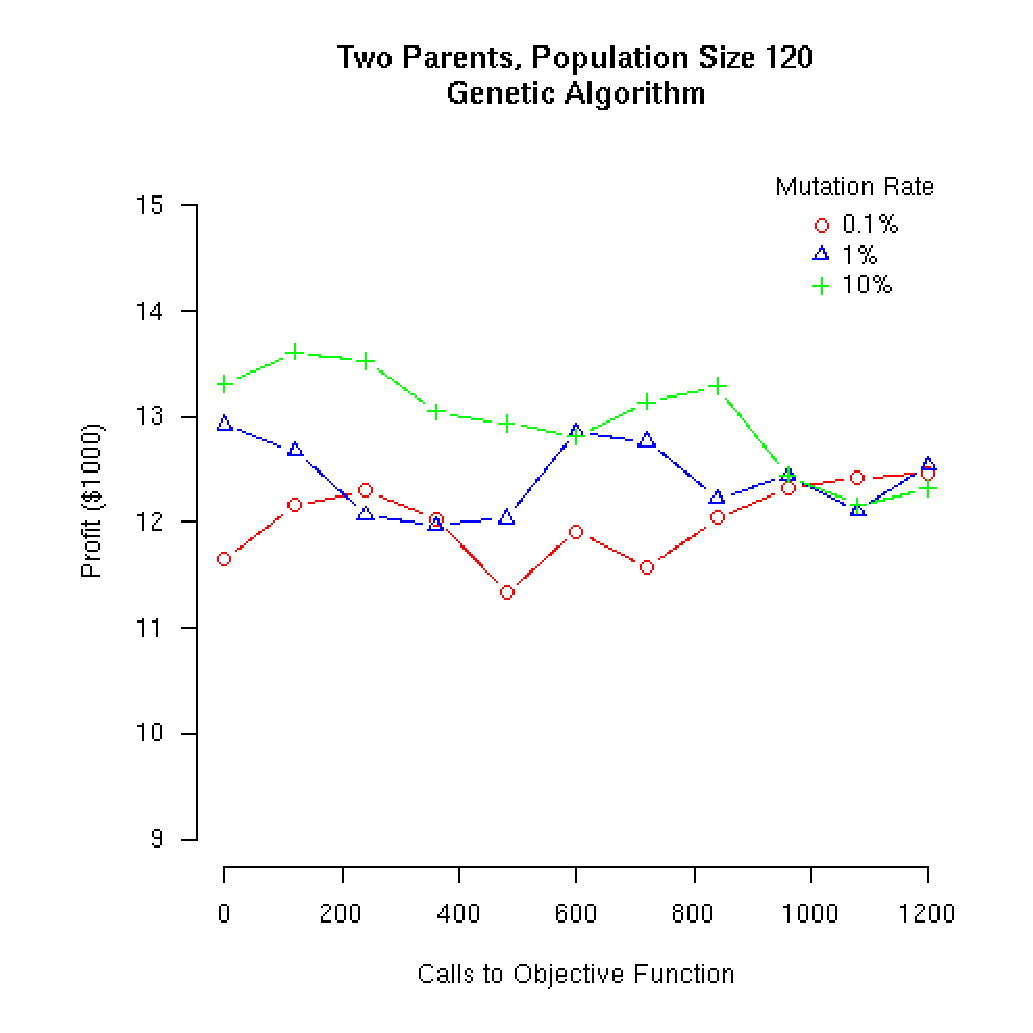
\includegraphics[width=7.5cm]{Gen2ParentsPop120.eps}
  \end{minipage}
  \begin{minipage}[b]{0.5\linewidth}
    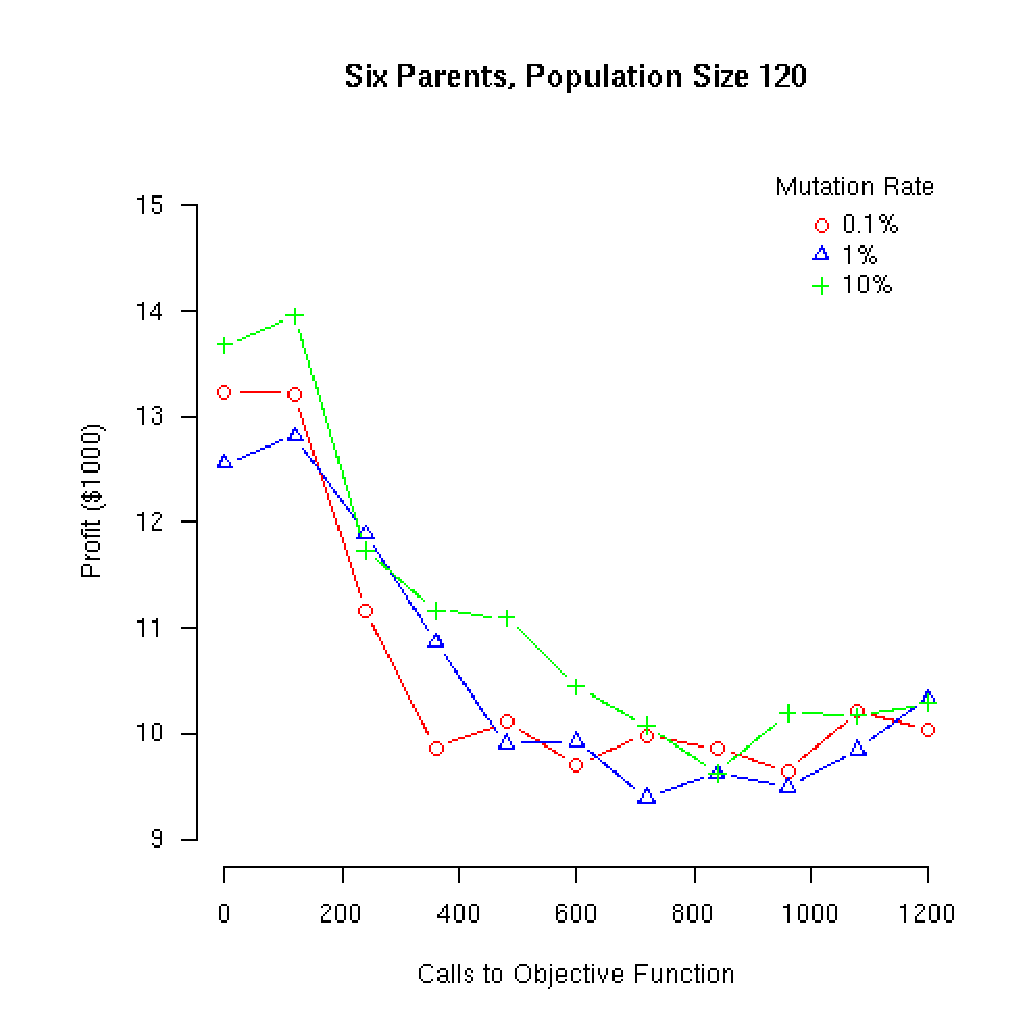
\includegraphics[width=7.5cm]{Gen6ParentsPop120.eps}
  \end{minipage}
  \begin{minipage}[b]{0.5\linewidth}
    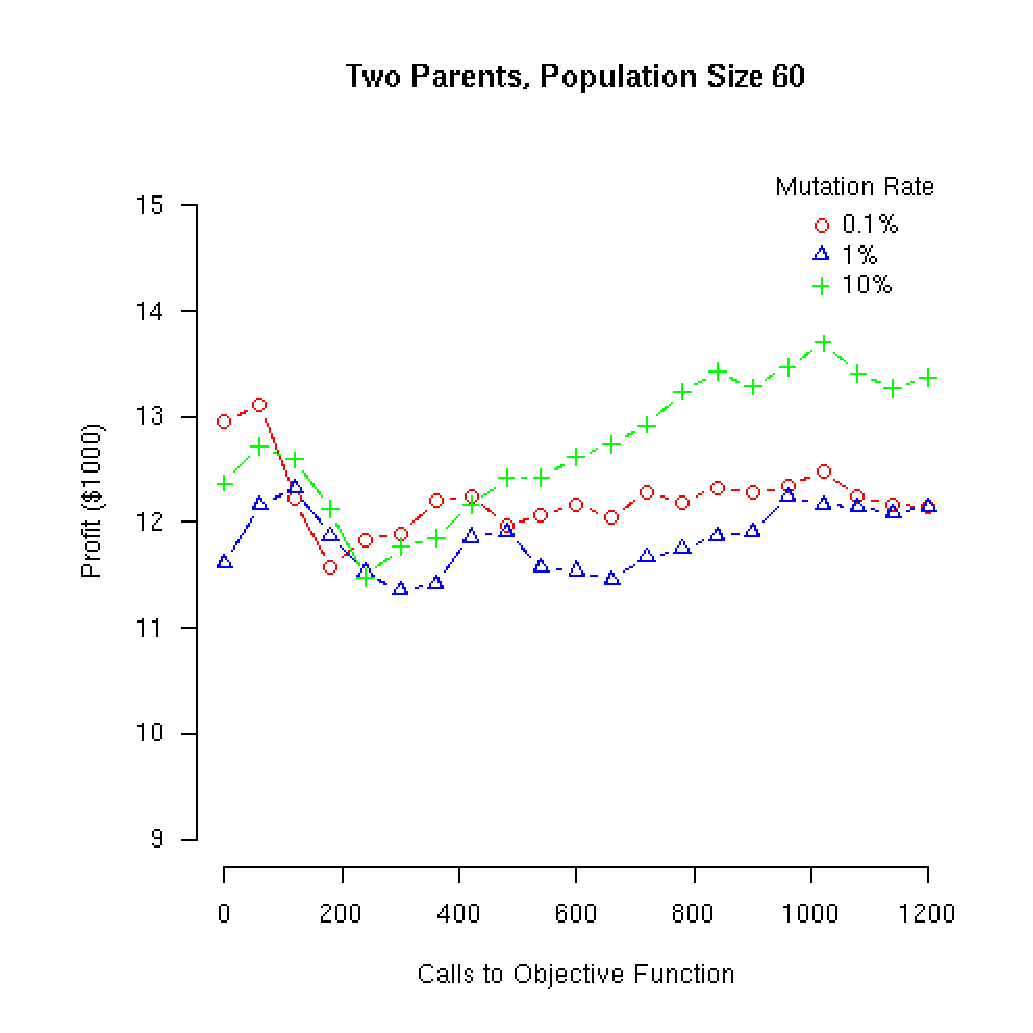
\includegraphics[width=7.5cm]{Gen2ParentsPop60.eps}
  \end{minipage}
  \begin{minipage}[b]{0.5\linewidth}
    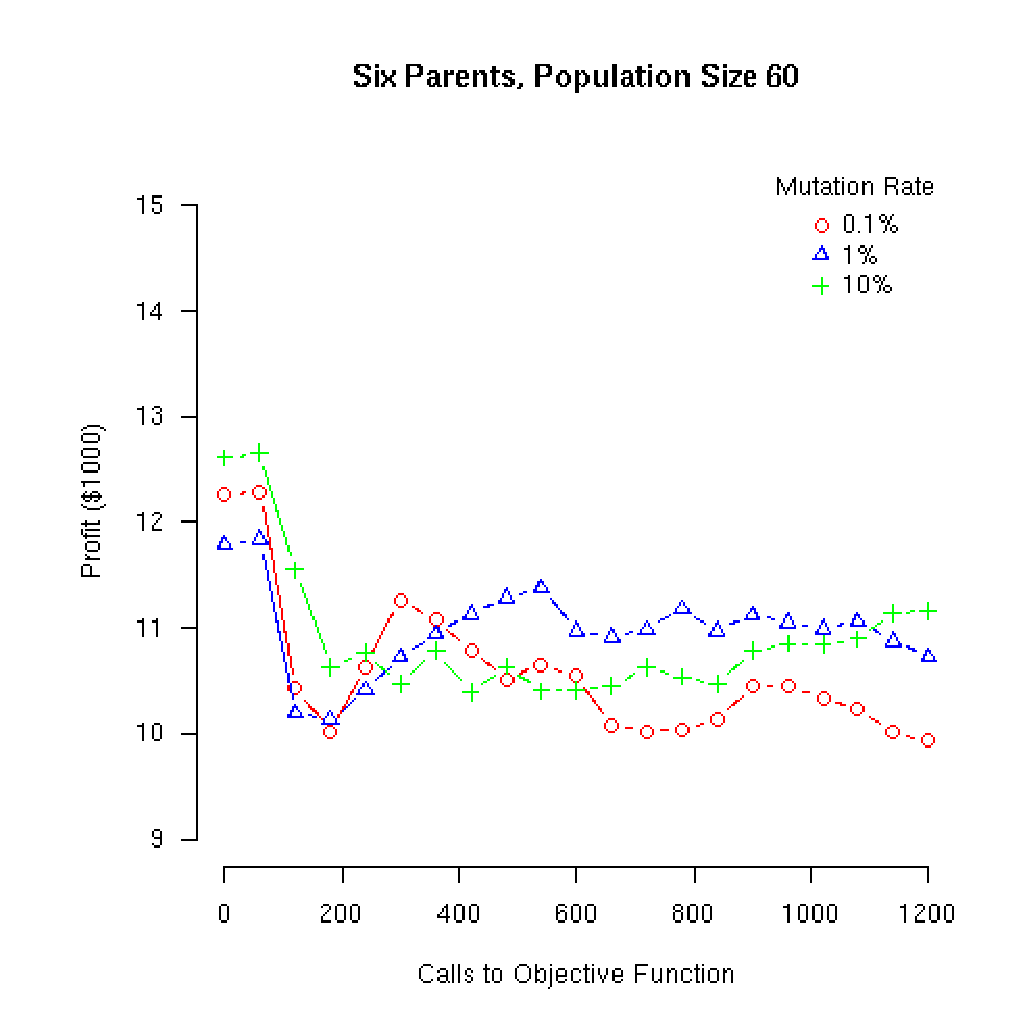
\includegraphics[width=7.5cm]{Gen6ParentsPop60.eps}
  \end{minipage}
  \begin{minipage}[b]{0.5\linewidth}
    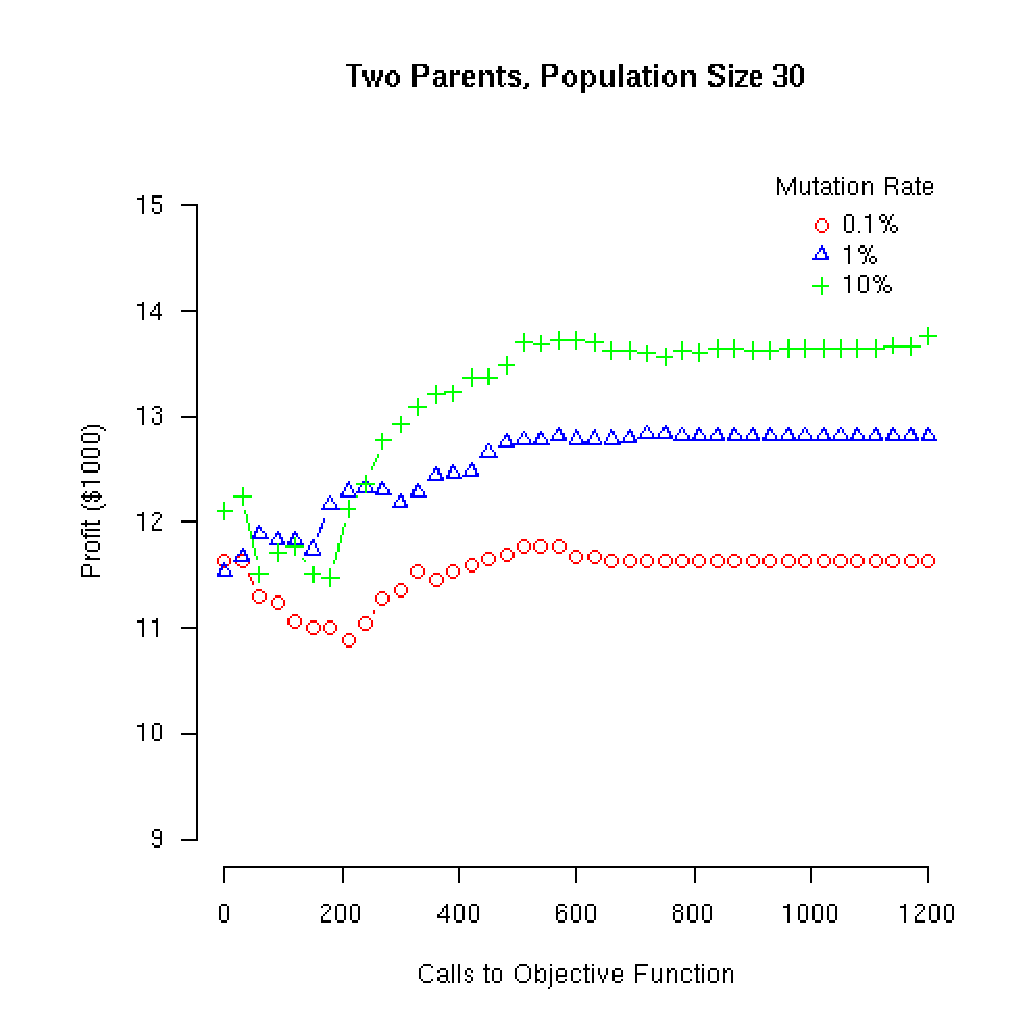
\includegraphics[width=7.5cm]{Gen2ParentsPop30.eps}
  \end{minipage}
  \begin{minipage}[b]{0.5\linewidth}
    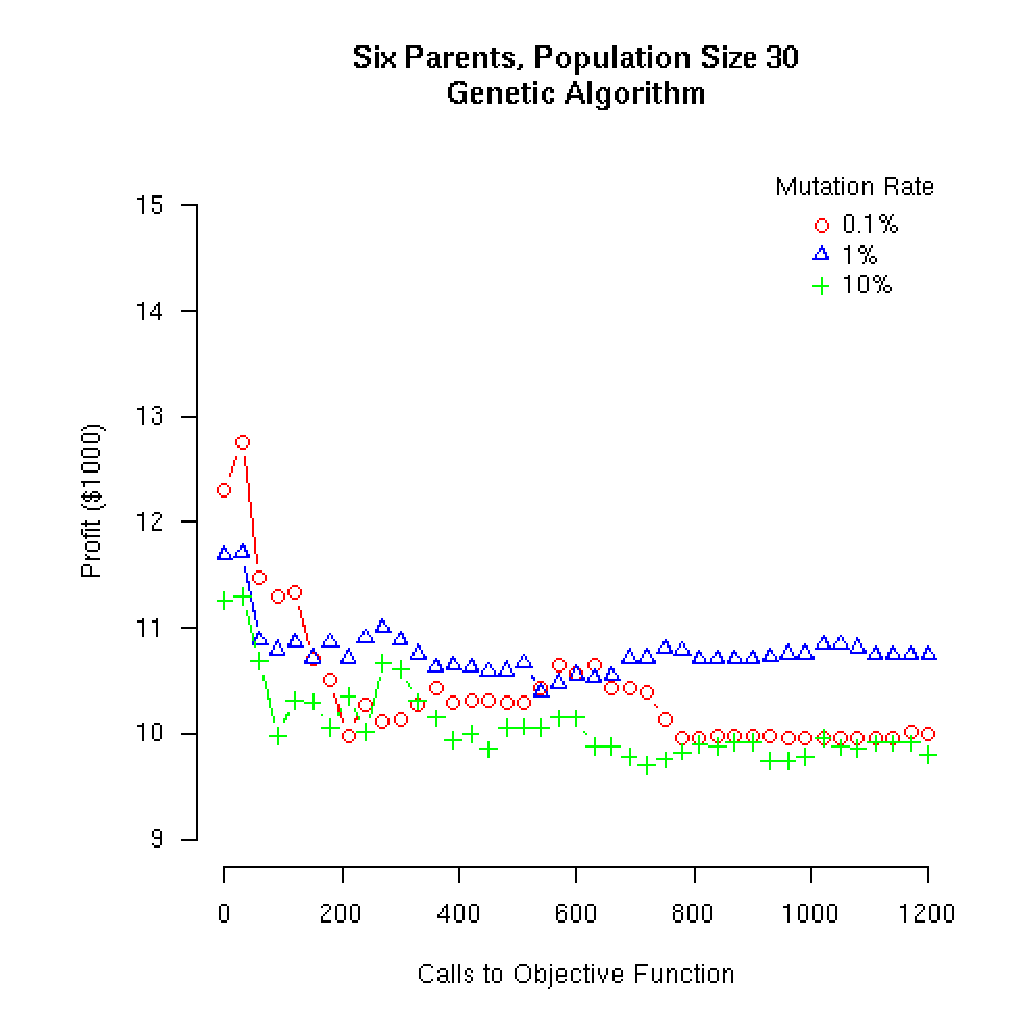
\includegraphics[width=7.5cm]{Gen6ParentsPop30.eps}
  \end{minipage}
\end{figure}

\pagebreak
\subsection{Successor Function}

\begin{figure}[!ht]
  \begin{minipage}[b]{0.5\linewidth}
    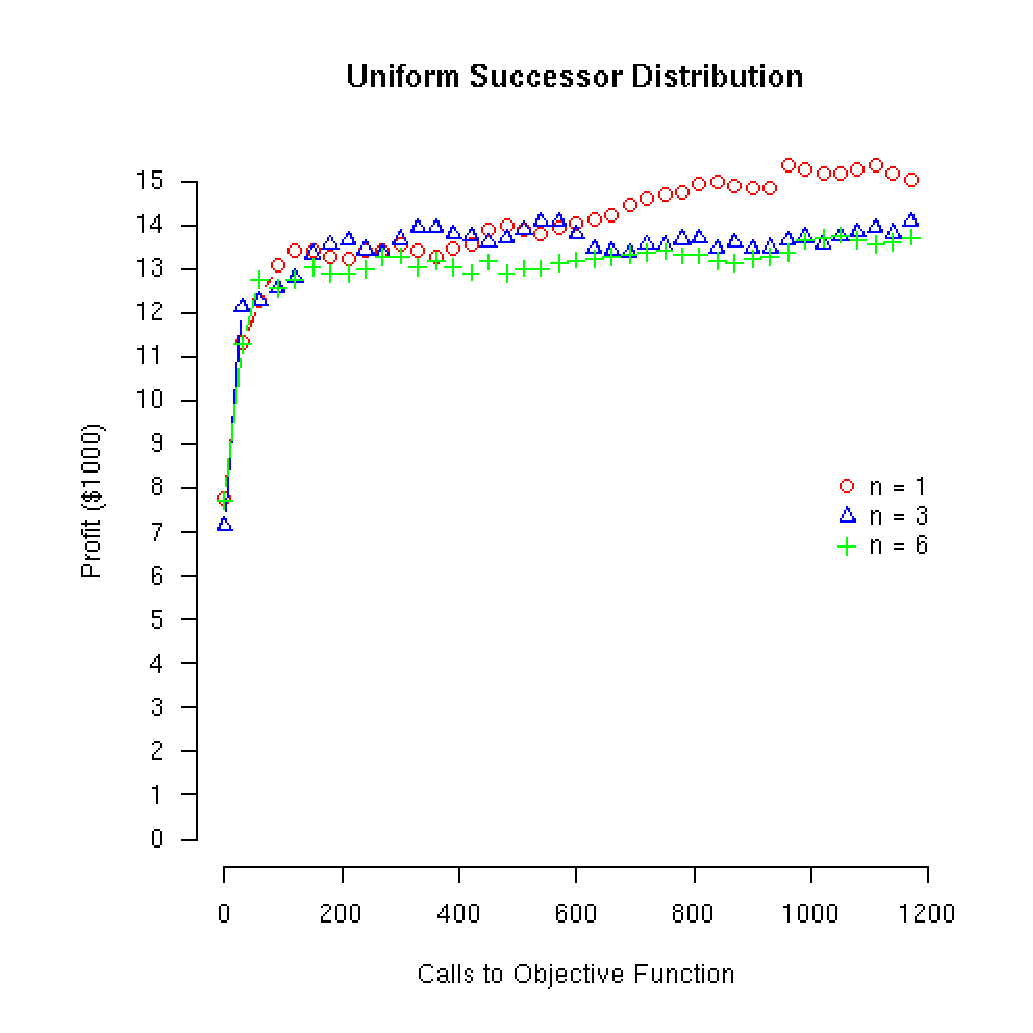
\includegraphics[width=7.5cm]{SimUNIFORMDist.eps}
  \end{minipage}
  \begin{minipage}[b]{0.5\linewidth}
    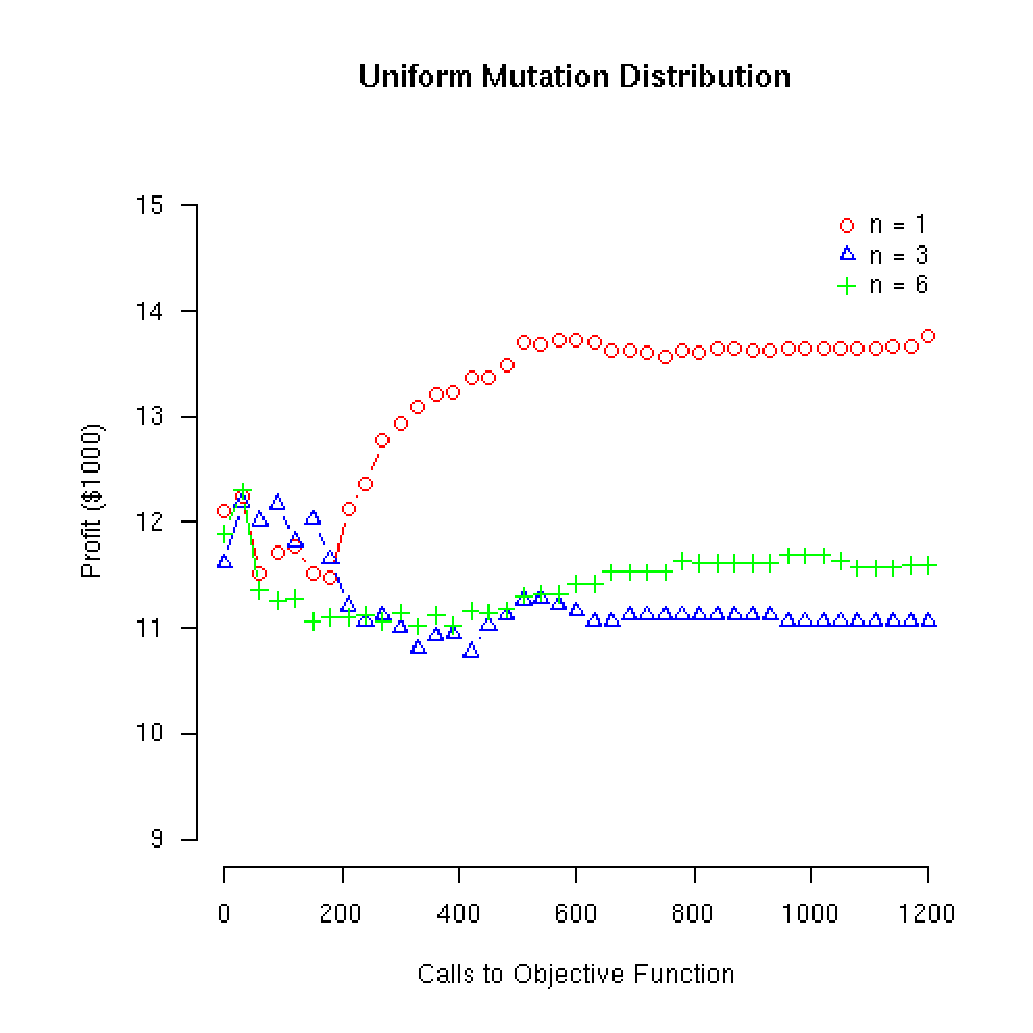
\includegraphics[width=7.5cm]{GenUNIFORMDist.eps}
  \end{minipage}
  \begin{minipage}[b]{0.5\linewidth}
    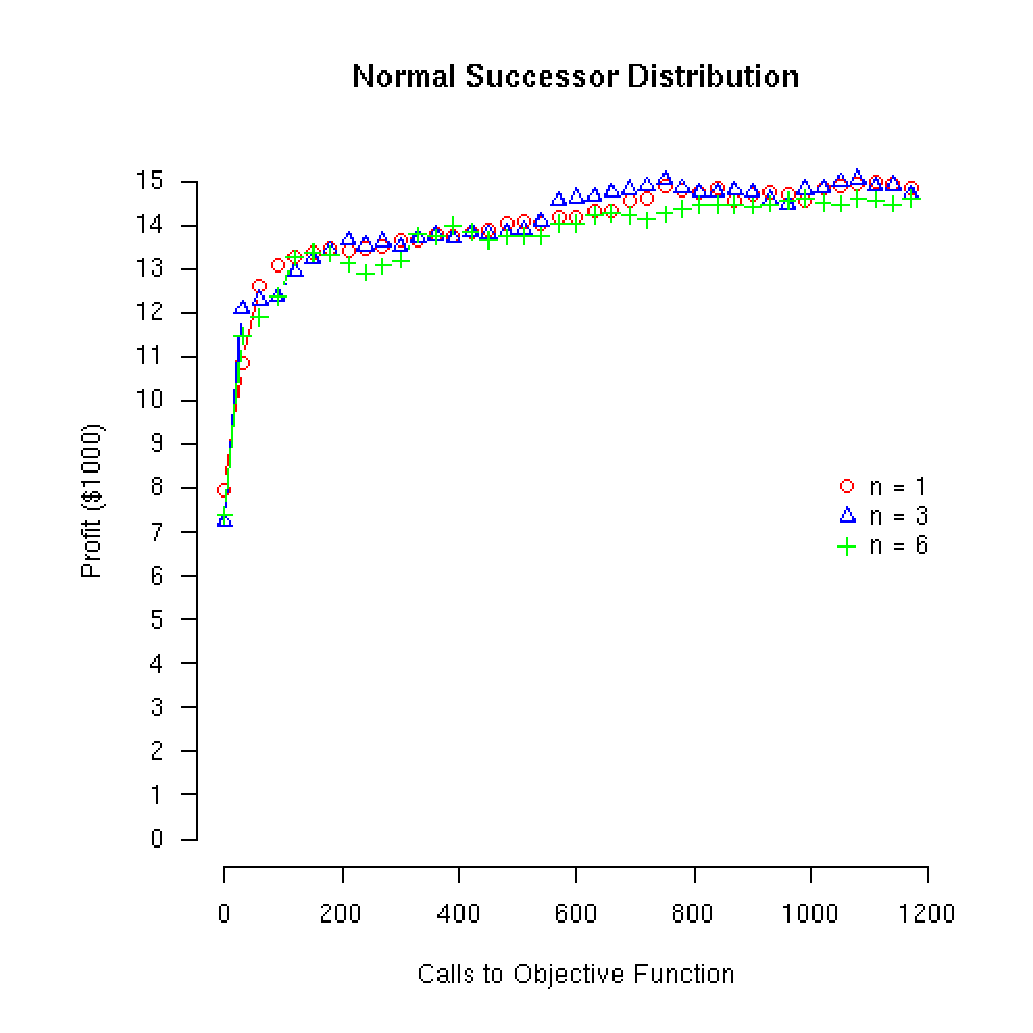
\includegraphics[width=7.5cm]{SimNORMALDist.eps}
  \end{minipage}
  \begin{minipage}[b]{0.5\linewidth}
    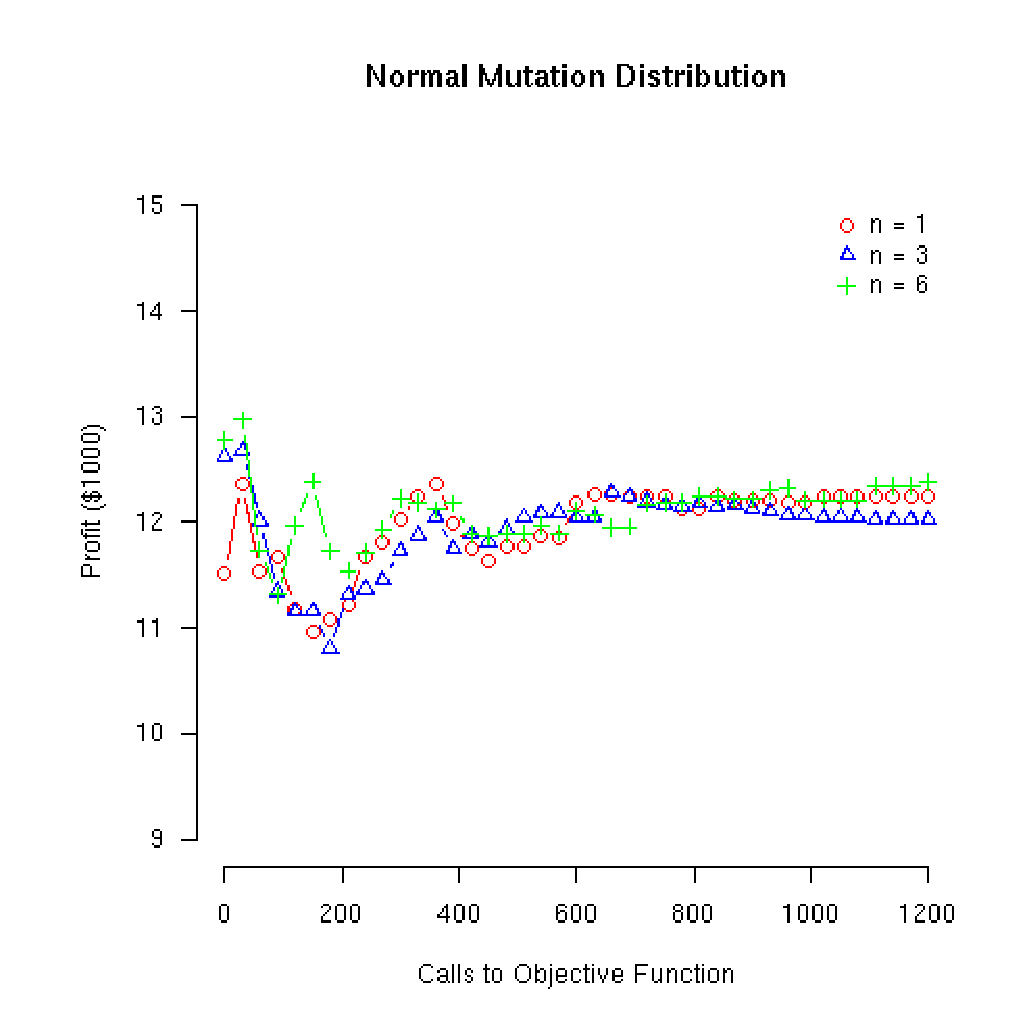
\includegraphics[width=7.5cm]{GenNORMALDist.eps}
  \end{minipage}
  \begin{minipage}[b]{0.5\linewidth}
    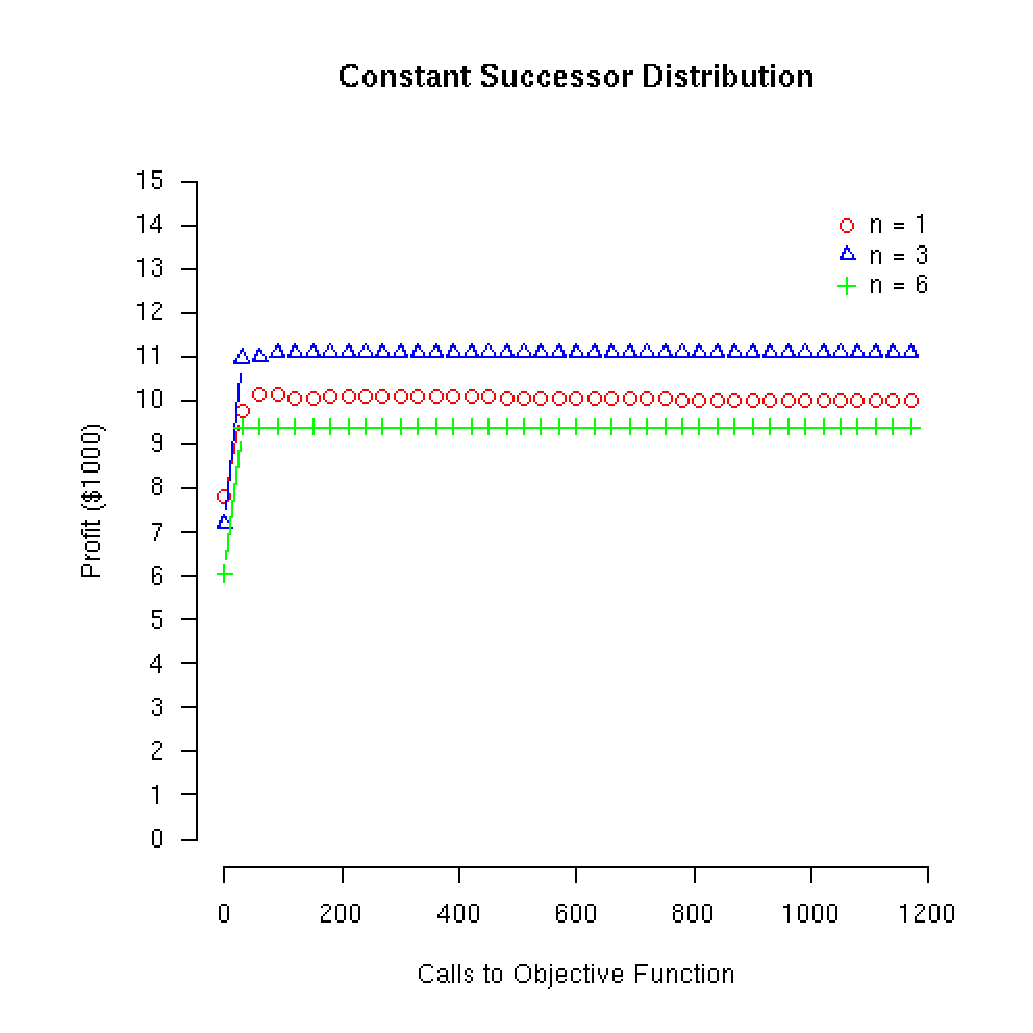
\includegraphics[width=7.5cm]{SimCONSTANTDist.eps}
  \end{minipage}
  \begin{minipage}[b]{0.5\linewidth}
    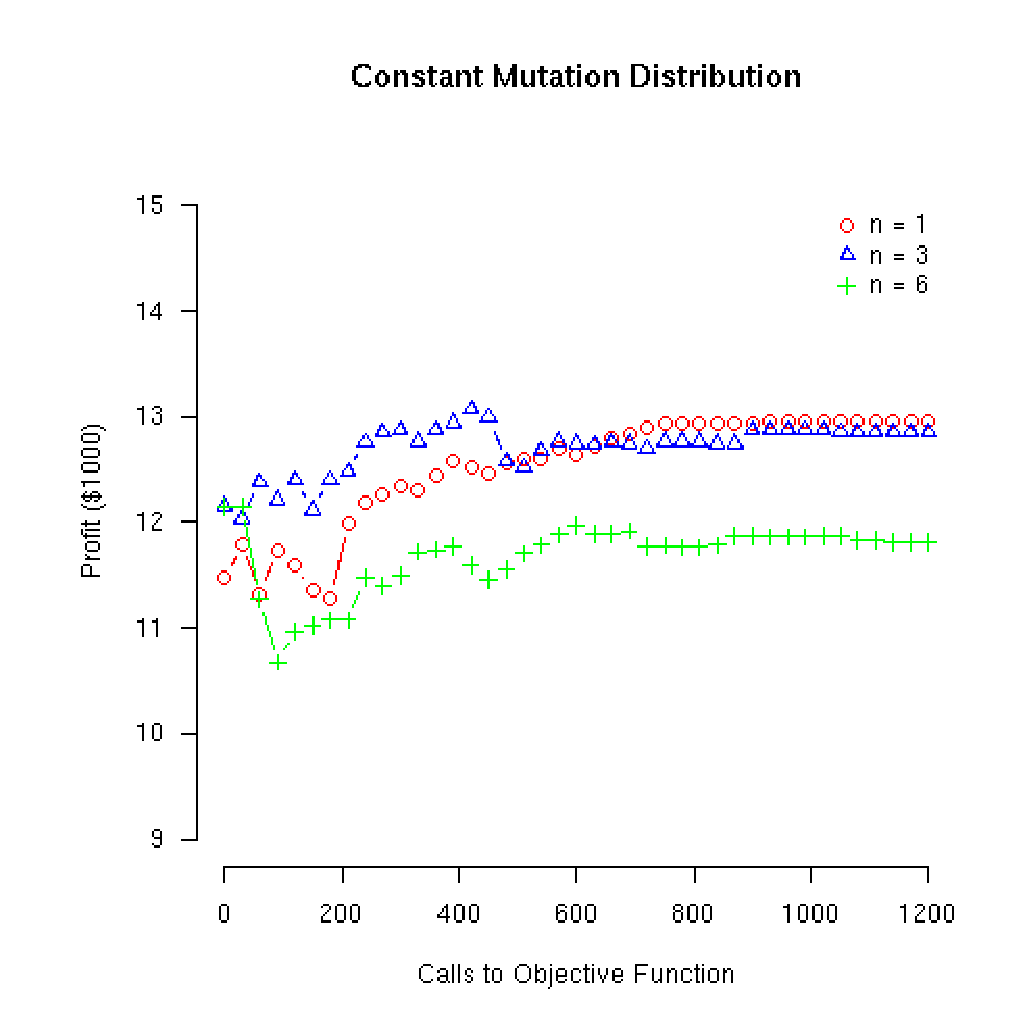
\includegraphics[width=7.5cm]{GenCONSTANTDist.eps}
  \end{minipage}
\end{figure}
\begin{figure}[!ht]
  \begin{minipage}[b]{0.5\linewidth}
    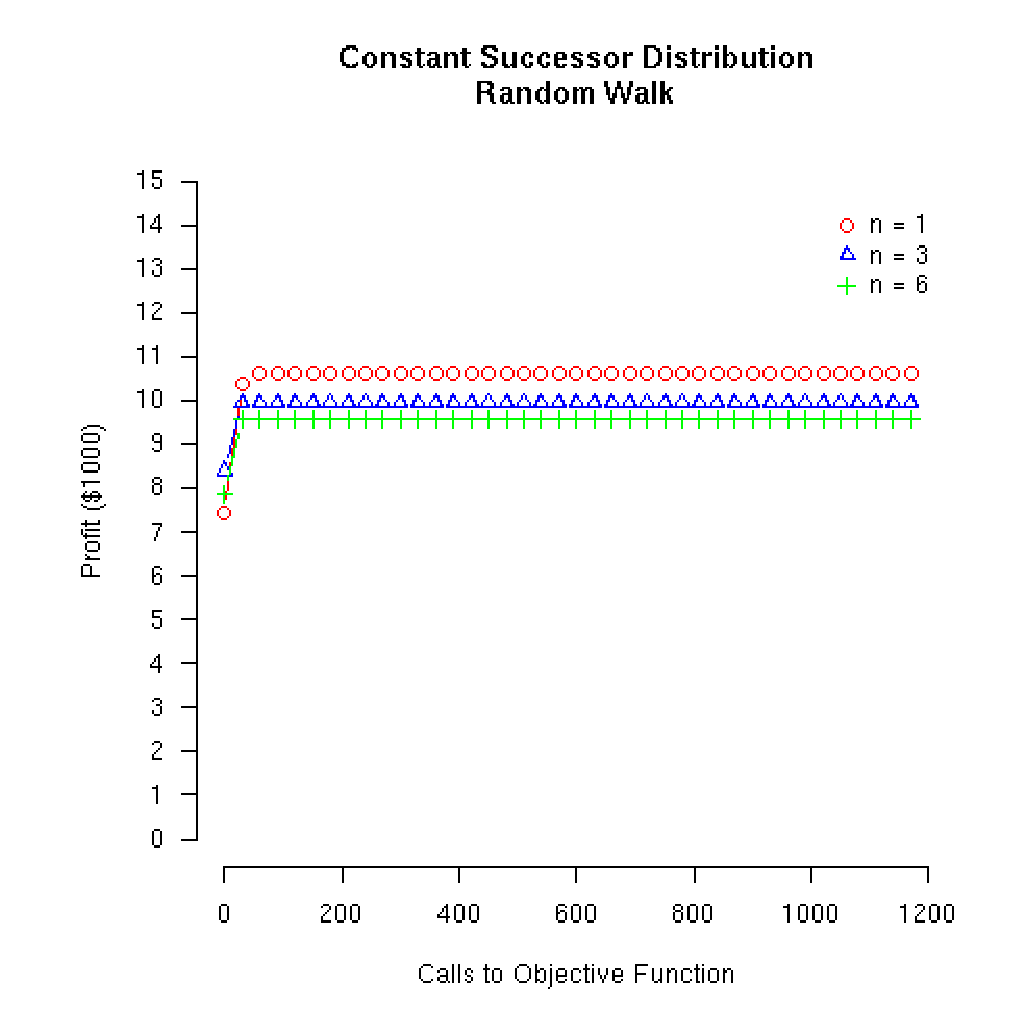
\includegraphics[width=7.5cm]{RanCONSTANTDist.eps}
  \end{minipage}
  \begin{minipage}[b]{0.5\linewidth}
    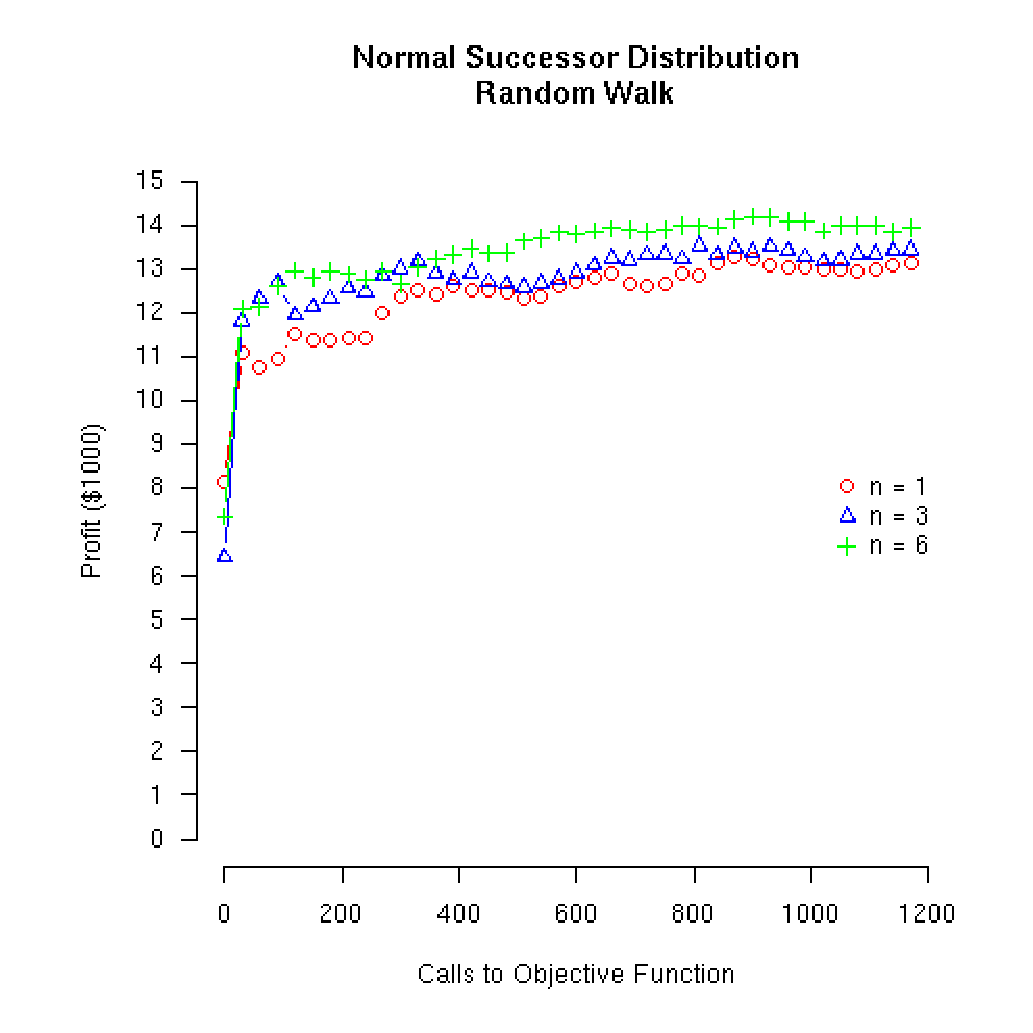
\includegraphics[width=7.5cm]{RanNORMALDist.eps}
  \end{minipage}
  \begin{minipage}[b]{0.5\linewidth}
    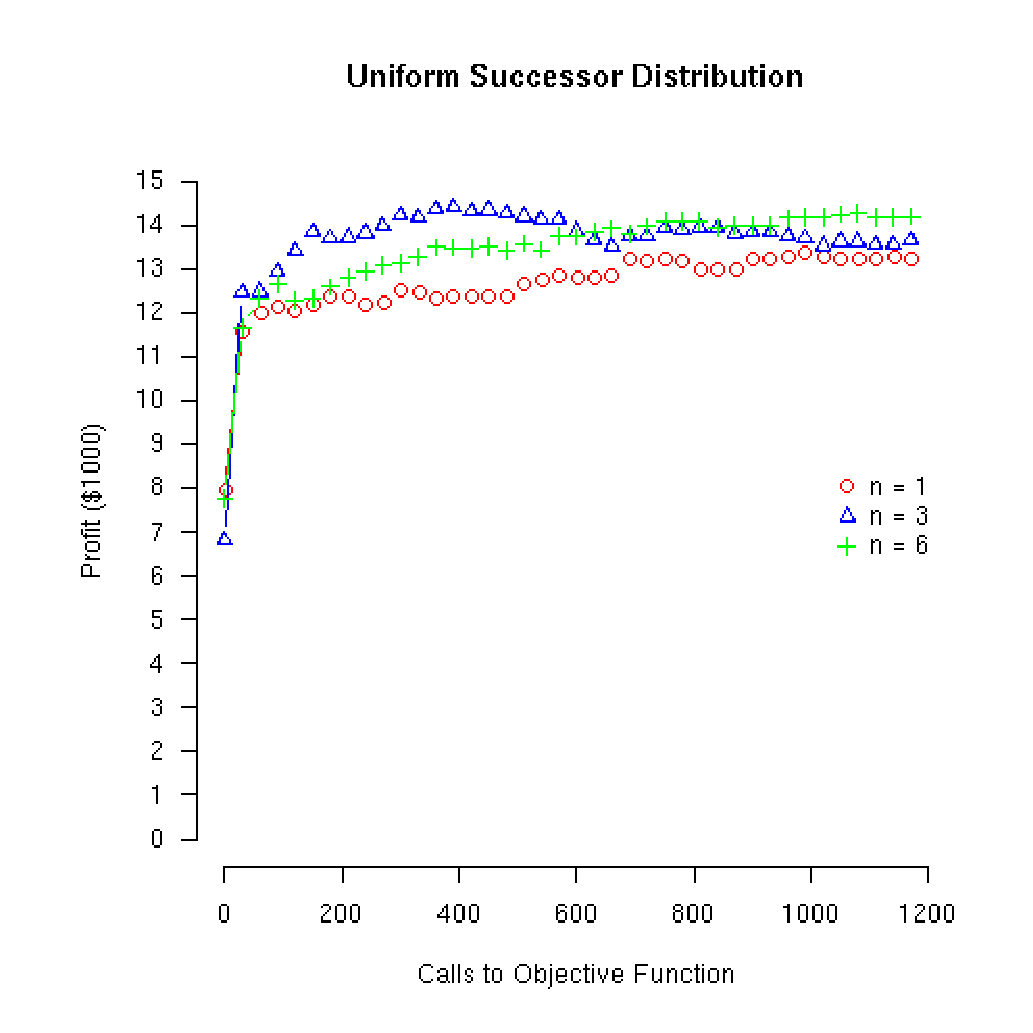
\includegraphics[width=7.5cm]{RanUNIFORMDist.eps}
  \end{minipage}
\end{figure}

\pagebreak
\subsection{Optimal Parameters}

\begin{tabular}{|r|l|l|l|l|l|l|l|}
  \hline
  April & \multicolumn{3}{|c|}{Channel Thresholds} & \multicolumn{3}{|c|}{Window Dates} &  \\
  Live Cattle & Entry & Trail Stop & Stop Loss & Open & Close & Exit & Profit\\ \hline
  Simulated Annealing & 9 & 10 & 6 & 04-21 & 03-18 & 04-07 & \$1,110.00 \\ \hline
  Genetic Algorithms & 45 & 31 & 39 & 03-23 & 01-22 & 02-19 & \$6,450.00 \\ \hline
  Random Walk & 2 & 13 & 34 & 06-20 & 04-12 & 03-07 & \$10,820.00 \\ \hline
  Momsen & 25 & 22 & 2 & 12-02 & 02-01 & 03-23 & \$4,740.00 \\ \hline
\end{tabular}

\begin{tabular}{|r|l|l|l|l|l|l|l|}
  \hline
  August & \multicolumn{3}{|c|}{Channel Thresholds} & \multicolumn{3}{|c|}{Window Dates} &  \\
  Pork Bellies & Entry & Trail Stop & Stop Loss & Open & Close & Exit & Profit\\ \hline
  Simulated Annealing & 3 & 4 & 35 & 10-19 & 08-27 & 01-02 & \$123,150.00 \\ \hline
  Genetic Algorithms & 7 & 3 & 39 & 04-16 & 12-29 & 05-31 & \$139,590.00 \\ \hline
  Random Walk & 1 & 49 & 16 & 01-09 & 10-13 & 04-09 & \$271,010.00 \\ \hline
  Momsen &  14 & 13 & 4 & 04-02 & 07-01 & 07-29 & \$30,030.00 \\ \hline
\end{tabular}

\begin{tabular}{|r|l|l|l|l|l|l|l|}
  \hline
  December & \multicolumn{3}{|c|}{Channel Thresholds} & \multicolumn{3}{|c|}{Window Dates} &  \\
  Corn & Entry & Trail Stop & Stop Loss & Open & Close & Exit & Profit\\ \hline
  Simulated Annealing & 4 & 27 & 23 & 03-21 & 01-01 & 12-19 & \$-3,138.00 \\ \hline
  Genetic Algorithms & 2 & 33 & 3 & 05-05 & 02-18 & 10-18 & \$97,793.50 \\ \hline
  Random Walk & 22 & 38 & 43 & 04-30 & 04-19 & 12-19 & \$541.50 \\ \hline
  Momsen & 21 & 11 & 2 & 05-12 & 08-01 & 08-06 & \$12,412.00 \\ \hline
\end{tabular}

\begin{tabular}{|r|l|l|l|l|l|l|l|}
  \hline
  December & \multicolumn{3}{|c|}{Channel Thresholds} & \multicolumn{3}{|c|}{Window Dates} &  \\
  Wheat & Entry & Trail Stop & Stop Loss & Open & Close & Exit & Profit\\ \hline
  Simulated Annealing & 2 & 12 & 3 & 01-25 & 01-01 & 12-19 & \$113,381.50 \\ \hline
  Genetic Algorithms & 17 & 12 & 44 & 06-12 & 02-21 & 07-21 & \$25,249.00 \\ \hline
  Random Walk & 1 & 27 & 21 & 08-23 & 08-12 & 08-30 & \$60,920.50 \\ \hline
  Momsen & 12 & 5 & 3 & 05-20 & 08-01 & 08-06 & \$9,925.00 \\ \hline
\end{tabular}

\begin{tabular}{|r|l|l|l|l|l|l|l|}
  \hline
  December  & \multicolumn{3}{|c|}{Channel Thresholds} & \multicolumn{3}{|c|}{Window Dates} &  \\
  Lean Hogs & Entry & Trail Stop & Stop Loss & Open & Close & Exit & Profit\\ \hline
  Simulated Annealing & 2 & 38 & 6 & 11-22 & 01-13 & 12-19 & \$131,680.00 \\ \hline
  Genetic Algorithms & 9 & 16 & 3 & 06-12 & 04-27 & 10-18 & \$108,960.00 \\ \hline
  Random Walk & 1 & 47 & 32 & 09-18 & 02-21 & 10-07 & \$62,310.00 \\ \hline
  Momsen & 12 & 12 & 5 & 05-15 & 07-01 & 08-12 & \$8,190.00 \\ \hline
\end{tabular}

\begin{tabular}{|r|l|l|l|l|l|l|l|}
  \hline
  February & \multicolumn{3}{|c|}{Channel Thresholds} & \multicolumn{3}{|c|}{Window Dates} &  \\
  Crude Oil & Entry & Trail Stop & Stop Loss & Open & Close & Exit & Profit\\ \hline
  Simulated Annealing & 2 & 40 & 25 & 05-30 & 03-28 & 06-24 & \$22,060.00 \\ \hline
  Genetic Algorithms & 9 & 12 & 3 & 03-10 & 02-21 & 07-21 & \$14,360.00 \\ \hline
  Random Walk & 1 & 46 & 17 & 08-16 & 01-30 & 08-29 & \$39,890.00 \\ \hline
  Momsen & 12 & 15 & 4 & 10-11 & 12-01 & 12-19 & \$11,440.00 \\ \hline
\end{tabular}

\begin{tabular}{|r|l|l|l|l|l|l|l|}
  \hline
  June & \multicolumn{3}{|c|}{Channel Thresholds} & \multicolumn{3}{|c|}{Window Dates} &  \\
  Crude Oil & Entry & Trail Stop & Stop Loss & Open & Close & Exit & Profit\\ \hline
  Simulated Annealing & 9 & 34 & 25 & 01-16 & 08-27 & 10-08 & \$16,290.00 \\ \hline
  Genetic Algorithms & 4 & 1 & 4 & 02-11 & 09-19 & 01-06 & \$10,830.00 \\ \hline
  Random Walk & 36 & 15 & 48 & 12-14 & 04-22 & 04-27 & \$9,390.00 \\ \hline
  Momsen & 17 & 14 & 3 & 02-24 & 04-01 & 04-20 & \$5,380.00 \\ \hline
\end{tabular}

\begin{tabular}{|r|l|l|l|l|l|l|l|}
  \hline
  June & \multicolumn{3}{|c|}{Channel Thresholds} & \multicolumn{3}{|c|}{Window Dates} &  \\
  Unleaded Gas & Entry & Trail Stop & Stop Loss & Open & Close & Exit & Profit\\ \hline
  Simulated Annealing & 3 & 17 & 21 & 05-31 & 04-25 & 09-24 & \$18,051.60 \\ \hline
  Genetic Algorithms & 32 & 15 & 12 & 07-15 & 11-24 & 05-16 & \$2,767.80 \\ \hline
  Random Walk & 31 & 49 & 31 & 07-26 & 03-18 & 05-09 & \$14,448.00 \\ \hline
  Momsen & 6 & 8 & 2 & 03-02 & 04-13 & 05-09 & \$13,679.00 \\ \hline
\end{tabular}

\begin{tabular}{|r|l|l|l|l|l|l|l|}
  \hline
  June & \multicolumn{3}{|c|}{Channel Thresholds} & \multicolumn{3}{|c|}{Window Dates} &  \\
  Lean Hogs & Entry & Trail Stop & Stop Loss & Open & Close & Exit & Profit\\ \hline
  Simulated Annealing & 13 & 27 & 19 & 05-30 & 03-31 & 05-26 & \$13,880.00 \\ \hline
  Genetic Algorithms & 32 & 25 & 39 & 07-15 & 05-21 & 06-01 & \$11,640.00 \\ \hline
  Random Walk & 1 & 17 & 25 & 08-18 & 03-17 & 05-24 & \$9,570.00 \\ \hline
  Momsen & 21 & 15 & 5 & 02-28 & 05-01 & 05-27 & \$4,260.00 \\ \hline
\end{tabular}

\begin{tabular}{|r|l|l|l|l|l|l|l|}
  \hline
  May & \multicolumn{3}{|c|}{Channel Thresholds} & \multicolumn{3}{|c|}{Window Dates} &  \\
  Heating Oil & Entry & Trail Stop & Stop Loss & Open & Close & Exit & Profit\\ \hline
  Simulated Annealing & 3 & 36 & 6 & 01-30 & 10-19 & 11-06 & \$14,082.60 \\ \hline
  Genetic Algorithms & 4 & 19 & 48 & 02-05 & 12-01 & 09-26 & \$15,808.80 \\ \hline
  Random Walk & 6 & 20 & 23 & 07-30 & 10-23 & 11-28 & \$3,570.00 \\ \hline
  Momsen & 23 & 9 & 2 & 02-24 & 04-01 & 04-20 & \$2,431.80 \\ \hline
\end{tabular}

\begin{tabular}{|r|l|l|l|l|l|l|l|}
  \hline
  November & \multicolumn{3}{|c|}{Channel Thresholds} & \multicolumn{3}{|c|}{Window Dates} &  \\
  Crude Oil & Entry & Trail Stop & Stop Loss & Open & Close & Exit & Profit\\ \hline
  Simulated Annealing & 18 & 24 & 11 & 12-05 & 08-11 & 10-08 & \$22,140.00 \\ \hline
  Genetic Algorithms & 27 & 23 & 8 & 12-13 & 08-31 & 10-15 & \$19,460.00 \\ \hline
  Random Walk & 24 & 24 & 49 & 1024 & 07-28 & 10-12 & \$34,710.00 \\ \hline
  Momsen & 10 & 5 & 3 & 07-24 & 09-05 & 09-25 & \$9,150.00 \\ \hline
\end{tabular}

\begin{tabular}{|r|l|l|l|l|l|l|l|}
  \hline
  November & \multicolumn{3}{|c|}{Channel Thresholds} & \multicolumn{3}{|c|}{Window Dates} &  \\
  Heating Oil & Entry & Trail Stop & Stop Loss & Open & Close & Exit & Profit\\ \hline
  Simulated Annealing & 3 & 20 & 19 & 03-13 & 10-30 & 10-09 & \$32,751.60 \\ \hline
  Genetic Algorithms & 16 & 1 & 12 & 12-13 & 09-03 & 09-29 & \$27,245.40 \\ \hline
  Random Walk & 2 & 7 & 42 & 02-27 & 09-17 & 05-25 & \$20,785.80 \\ \hline
  Momsen &  19 & 11 & 5 & 07-02 & 09-30 & 10-08 & \$13,981.80 \\ \hline
\end{tabular}

\begin{tabular}{|r|l|l|l|l|l|l|l|}
  \hline
  October & \multicolumn{3}{|c|}{Channel Thresholds} & \multicolumn{3}{|c|}{Window Dates} &  \\
  Lean Hogs & Entry & Trail Stop & Stop Loss & Open & Close & Exit & Profit\\ \hline
  Simulated Annealing & 5 & 34 & 25 & 10-19 & 10-14 & 10-08 & \$-13,250.00 \\ \hline
  Genetic Algorithms & 24 & 32 & 12 & 12-13 & 09-22 & 09-28 & \$5,050.00 \\ \hline
  Random Walk & 5 & 29 & 34 & 12-19 & 09-05 & 09-23 & \$3,690.00 \\ \hline
  Momsen & 15 & 7 & 1 & 08-29 & 09-30 & 10-01 & \$6,360.00 \\ \hline
\end{tabular}

\begin{tabular}{|r|l|l|l|l|l|l|l|}
  \hline
  September    & \multicolumn{3}{|c|}{Channel Thresholds} & \multicolumn{3}{|c|}{Window Dates} &  \\
  Orange Juice & Entry & Trail Stop & Stop Loss & Open & Close & Exit & Profit\\ \hline
  Simulated Annealing & 4 & 12 & 27 & 01-30 & 01-21 & 06-19 & \$71,677.50 \\ \hline
  Genetic Algorithms & 30 & 14 & 8 & 04-18 & 03-18 & 06-16 & \$-2,347.50 \\ \hline
  Random Walk & 5 & 34 & 27 & 10-03 & 09-22 & 11-01 & \$77,257.50 \\ \hline
  Momsen & 10 & 7 & 3 & 05-02 & 06-15 & 06-26 & \$1,890.00 \\ \hline
\end{tabular}

\bibliographystyle{plain}
\bibliography{final}
\nocite{*}
\end{document}
\end
